\chapter{Sucesiones de Mayer-Vietoris}\label{MVTema}
Sea $X$ un espacio topológico, $A \subseteq X$ un subespacio topológico y $\mathcal{U}$ una familia de subconjuntos de $X$ cuyos interiores formen un recubrimiento de $X$. Denotaremos a la familia de todos los interiores como $\mathcal{U}^o$
\\

Se define el grupo $S^\mathcal{U}_n(X)$ como el subgrupo de $S_n(X)$ generado por aquellos símplices $\phi: \sigma_n \rightarrow X$ tales que $$\exists U \in \mathcal{U}: \phi(\sigma_n) \subset U$$ Dado un $0 \leq i \leq n$, se tiene que $$\partial_{(i)}\phi(\sigma_{p-1}) \subset \phi(\sigma_p) \implies \phi \in S^U_p(X) \implies \partial_{(i)}\phi \in S^U_{p-1}(X)$$ Por tanto, la aplicación $\partial: S^U_n(X) \longrightarrow S^U_{n-1}(X)$ está bien definida y $S^\mathcal{U}_*(X)$ define un complejo de cadenas tomando $\partial$ como operador borde. Además, la inclusión $i: S^\mathcal{U}_*(X) \hookrightarrow S_*(X)$ es una aplicación de cadenas.
\\

Sea $\mathcal{V}$ un recubrimiento de $Y \in \topo$ tal que $\mathcal{V}^o$ también forma un recubrimiento de $Y$ y $f: X \longrightarrow Y$ una aplicación continua tal que $$\forall U \in \mathcal{U}\; \exists V \in \mathcal{V}:\; f(U)\subseteq V$$ Bajo esta premisa, si $U \in \mathcal{U}$ y $\phi: \sigma_p \rightarrow U$, existirá un $V \in \mathcal{V}$ tal que $f_\#(\phi)(\sigma_p) \subseteq V$, por lo que $f$ induce una aplicación de cadenas $$f_\#: S^\mathcal{U}_*(X) \longrightarrow S^\mathcal{V}_*(Y)$$ que conmuta con la inclusión.
\\

\begin{teo}\label{IncIso}
Sea $X \in \topo$ y $\m{U}$ un recubrimiento de $X$ tal que $\m{U}^o$ también es recubrimiento de $X$. La aplicación $i_*: H_n(S_n^\m{U}(X)) \longrightarrow H_n(X)$ es un isomorfismo.
\end{teo}

Considérese el caso más sencillo: sean $U,V \subset X$ tales que $$\mbox{int}(U) \cap \mbox{int}(V)=X$$
y $\m{U}=\{U,V\}$. Si denotamos como $A$ al conjunto de $n$-símplices singulares sobre $U$ y como $B$ al conjunto de $n$-símplices singulares sobre $V$, tenemos que $$S_n(U)=F(A); \quad S_n(V)=F(B);$$ $$S_n(U \cap V)=F(A \cap B); \quad S_n(X)=F(A \cup B)$$

Consideremos el epimorfismo
\[\begin{array}{cccc}
h:& F(A) \oplus F(B)& \longrightarrow& F(A\cup B)\\
  & (a,b)           & \longmapsto    & a+b
\end{array}\]
y el monomorfismo
\[\begin{array}{cccc}
g:& F(A\cap B)& \longrightarrow& F(A)\oplus F(B)\\
  & f           & \longmapsto    & (f,-f)
\end{array}\]
La secuencia $$0 \longrightarrow S_n(U \cap V) \xrightarrow{ g } S_n(U)\oplus S_n(V) \xrightarrow{ h } S_n^\m{U}(X) \longrightarrow 0$$ es una sucesión exacta corta.

\begin{proof}
Dado un $c \in F(A \cup B)$, se tiene que $$(h\circ g)(c)=h(c,-c)=c-c=0 \implies \im g \leq \ker h$$ Ahora bien: sean $a \in F(A)$ y $b \in F(B)$ tales que $$a+b=h(a,b)=0 \iff a=-b$$ Dado que $F(A)$ y $F(B)$ son grupos libres, se tiene que $a$ puede ser escrito como combinación lineal de elemenos de $A$ y de elementos de $B$ al mismo tiempo.
\\

Por tanto, $a \in F(A\cap B)$. Además, como $a=-b$, se cumple que $$(a,b)=(a,-a)=g(a)$$ por lo que $\ker k \leq \im g$. Se sigue que $\ker k = \im g$.
\end{proof}

Se define $S_*(U)\oplus S_*(V):=\{S_n(U)\oplus S_n(V): \; n \in \mb{Z}\}$, de forma que la sucesión exacta anterior da lugar a la sucesión exacta $$0 \longrightarrow S_*(U \cap V) \xrightarrow{ g } S_*(U)\oplus S_*(V) \xrightarrow{ h } S^\m{U}_*(X) \longrightarrow 0$$

Vamos a aplicar el teorema \ref{SucExacHomo} para obtener una sucesión exacta larga en homología a partir de esta sucesión exacta corta. Para ello, observar que $$H_n(S_*(U)\oplus S_*(V))\cong H_n(S_*(U))\oplus H_n(S_*(V))\cong H_n(U)\oplus H_n(V)$$ Además, el teorema \ref{IncIso} nos dice que $H_n(S^\m{U}_*(X)) \cong H_n(X)$.
\\

\cuadro{Sea $X$ un espacio topológico y $U,V \subset X$ subespacios tales que $X=\mbox{int}(U)\cup \mbox{int}(V)$. Si $\Delta: H_*(X) \longrightarrow H_*(U \cap V)$ es el homomorfismo de conexión, se define la \textbf{sucesión de Mayer-Vietoris} asociada al par $\{U,V\}$ como la sucesión exacta larga $$H_n(U \cap V) \xrightarrow{ g_* } H_n(U)\oplus H_n(V) \xrightarrow{ h_* } H_n(X) \xrightarrow{ \Delta } H_{n-1}(U \cap V)$$}

El siguiente resultado establece una condición suficiente para saber cuándo dos 1-símplices singulares son homólogos.

\begin{lema}[Homotópico implica homólogo]
Sean $f,g: [0,1] \longrightarrow X$ dos caminos cerrados y homotópicos. $$f+B_1(X)=g+B_1(X)$$
\end{lema}

\begin{proof}
Como sabemos por el ejemplo \ref{Camino1ciclo}, $f$ y $g$ se identifican con 1-ciclos de $X$ por ser caminos cerrados, por lo que $f,g \in Z_1(X)$. Sea $$F: [0,1]^2 \longrightarrow X$$ una aplicación continua tal que $$F(0,t)=f(t); \quad F(1,t)=g(t) \quad \forall t \in [0,1]$$

Sea $\sim$ la relación de equivalencia que relaciona los puntos $(t,0)$ y $(t,1)$, con $t \in [0,1]$. Claramente, el espacio topológico cociente $C=[0,1]^2/\sim$ es un cilindro plano, que podemos considerar como variedad con borde.
\\

Considérese la aplicación
\[\begin{array}{cccc}
F_C:&C	  &\longrightarrow&X	 \\
	&(u,v)&\longmapsto	  &F(u,v)
\end{array}\]
Podemos identificar $F$ con $F_C$ sin pérdida de generalidad, dado que $f(0)=f(1)$ y $g(0)=g(1)$ por hipótesis. Por tanto, de ahora en adelante, trabajaremos sobre $C$ y su representación plana en lugar de trabajar sobre $[0,1]^2$.
\\

Si dibujamos sobre $C$ un segmento que una los puntos $[(1,0)]$ y $[(0,1)]$, tendremos a $C$ dividido en dos triángulos, a los que llamaremos $A$ y $B$ (ver figura).

\begin{figure}[h]
\centering
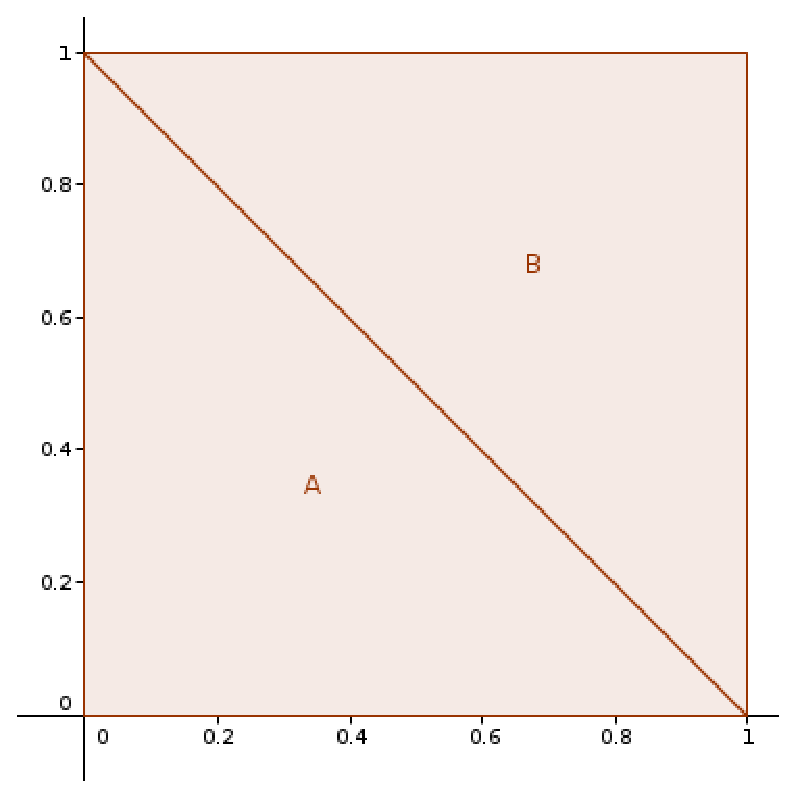
\includegraphics[scale=0.4]{Ej3paso1.eps}
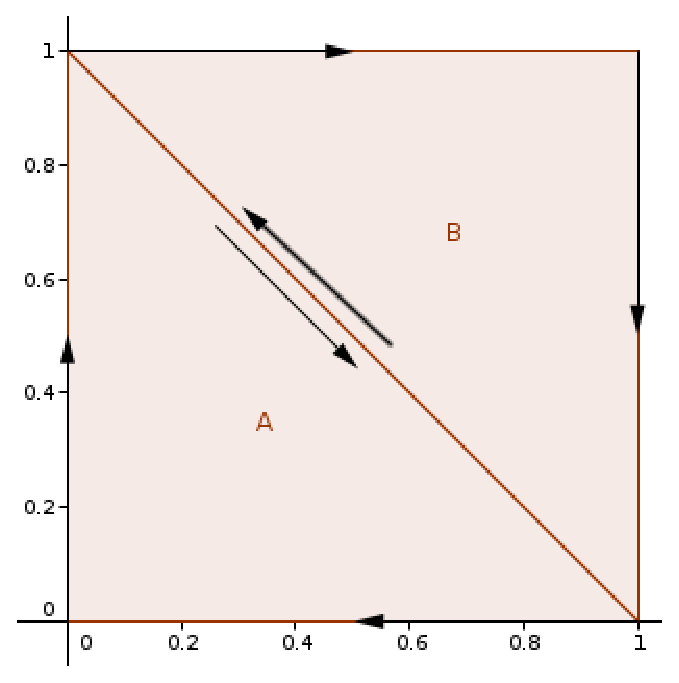
\includegraphics[scale=0.475]{Ej3paso2.eps}
\caption{$C$ queda dividido en dos triángulos, $A$ y $B$, a los cuales asignamos orientaciones contrarias orientando los bordes en direcciones opuestas.}
\end{figure}

Asignaremos a los segmentos $[(0,t)]$ y $[(1,t)]$ orientaciones contrarias. Estas orientaciones nos permiten orientar de forma única $A$ y $B$ a partir de sus bordes (ver figura 1).
\\

Definimos los 2-símplices singulares
\[\begin{array}{cccc}
\alpha:& \sigma_2 &\longrightarrow &C\\
            &(t_0,t_1,t_2)&\mapsto             &[(t_0,t_1)]
\end{array}\]

\[\begin{array}{cccc}\beta:& \sigma_2 &\longrightarrow &C\\
            &(t_0,t_1,t_2)&\mapsto             &[(t_0+t_1,t_0+t_2)]
\end{array}\]

Teniendo en cuenta que $(t,0)\sim (t,1)$ para todo $t \in [0,1]$,
\begin{align*}
\partial(\beta-\alpha)&(t_0,t_1)=\\
             &=[(t_0,t_1)]-[(t_0,t_1)]-[(t_0,1)]+[(1,t_0)]-[(0,t_0)]+[(t_0,0)]=\\
             &=[(1,t_0)]-[(0,t_0)]+[(t_0,0)]-[(t_0,0)]=\\
             &=[(1,t_0)]-[(0,t_0)]
\end{align*}

Dado que $F$ es una aplicación continua, induce una aplicación de cadenas $F_\#: S_*(C) \rightarrow S_*(X)$.
\begin{align*}
\partial [F_\#(\gamma-\alpha)](t_0,t_1)=&F_\#[\partial(\beta- \alpha)](t_0,t_1)=\\
                                       =&F(1,t_0)-F(0,t_0)=f(t_0)-g(t_0)
\end{align*}

Dado que $F_\#(\gamma-\alpha)=F_\#(\gamma)-F_\#(\alpha)$ es un 2-símplice singular de $X$, se deduce que $$f-g \in B_1(X) \iff f+B_1(X)=g+B_1(X)$$ Por tanto, $f$ y $g$ son caminos homólogos.\end{proof}

\section{Grupo de homología de $S^1$}
Sean $U=S^1-\{(1,0)\}$ y $V=S^1-\{(-1,0)\}$. Tenemos que $U\cap V$ es la unión disjunta de dos arcos de circunferencia, $C_1$ y $C_2$, que son conjuntos arcoconexos. Aplicando la proposición \ref{SumaDirArco}, se tiene que $$H_n(U\cap V) \cong H_n(C_1)\oplus H_n(C_2)$$ para todo $n \geq 0$.
\\

Dado que $C_1$ y $C_2$ son curvas cerradas y simples, son homeomorfas a un intervalo abierto $I \subset \mbR$ arbitrario, por lo que $$H_n(C_1) \cong H_n(I) \cong H_n(C_2)$$ Pero claro, los intervalos son conjuntos convexos, por lo que se deduce de la proposición \ref{Convexo} que $H_n(I)=0$ para todo $n > 0$ y $H_0(I)\cong\mb{Z}$.
\\

Combinando toda esta información, concluimos que $$H_n(U\cap V) \cong H_n(C_1)\oplus H_n(C_2) \cong H_n(I)^2 \cong \begin{cases}\mb{Z}^2 &\mbox{ si } n =0 \\ 0 &\mbox{ si no}\end{cases}$$

Por otro lado, $U$ y $V$ también son homeomorfos a un intervalo abierto de la recta real, por lo que podemos aplicar el mismo razonamiento para concluir que $$H_n(U) \cong 0 \cong H_n(V)\quad (n > 0)$$ y que $H_0(V) \cong \mb{Z} \cong H_0(U)$.
\\

Consideremos el siguiente tramo de la sucesión de Mayer-Vietoris asociada a este recubrimiento, donde las flechas verticales indican isomorfismos.
\[\begin{array}{ccccc}
H_1(U)\oplus H_1(V)	&\xrightarrow{h_1}	&H_1(S^1)		&\xrightarrow{\Delta_1}&H_0(U \cap V)\\
\downarrow			&					&\downarrow	&					&\downarrow\\
0			&\rightarrow			&H_1(S^1)		&\rightarrow			&\mb{Z}^2
\end{array}\]

Como la sucesión es exacta, $\im h_1=0$, luego $\ker_1 \Delta = \im h_1=0$, de forma que $\Delta$ es un monomorfismo. Se sigue que $$H_1(S^1)\cong \im \Delta = \ker g_1 \leq H_0(U\cap V)\cong \mb{Z}^2$$

Como $H_1(S^1) \cong \ker g_*$, podemos calcular dicho grupo estudiando cómo se comporta el homomorfismo $g_*$.
\\

Sea $w \in Z_0(U \cap V)$ y $[w]$ su clase módulo $B_0(U \cap V)$. Existirán $x,y \in U \cap V$, uno en cada componente conexa, y $a,b \in \mb{Z}$ tales que $$[w]=[ax+by]$$ Considérense las aplicaciones inclusión $$i_*: H_0(U \cap V) \hookrightarrow H_0(U); \quad j_*: H_0(U \cap V) \hookrightarrow H_0(V)$$ Si $[w] \in \ker g_*$, se tiene que
$$0=g_*([w])=(i_*([w]),-j_*([w])) \iff
\begin{cases}
i_*([w])=0\\
j_*([w])=0
\end{cases}$$
Pero $i_*([w]) \in H_0(U)$, por lo que $i_*([x])$ es homólogo a $i_*([y])$ y $$0=i_*([ax+by])=i_*([ax+bx])=(a+b)i_*([x]) \iff a+b=0$$ De aquí se tiene entonces que los elementos de $\ker g_*$ son de la forma $[ax-ay]$ con $a \in \mb{Z}$. Por tanto, $$H_1(S^1) =\ker g_*=\la[x-y]\ra \cong \mb{Z}$$

Sea $n > 1$. Se tiene la sucesión exacta
\[\begin{array}{ccccc}
H_n(U)\oplus H_n(V)	&\xrightarrow{h_n}	&H_n(S^1)		&\xrightarrow{\Delta_n}&H_{n-1}(U \cap V)\\
\downarrow	&					&\downarrow&&\downarrow\\
0			&\rightarrow			&H_n(S^1)		&\rightarrow			&0
\end{array}\]

Como esta sucesión es exacta, $\ker \Delta_n=\im h_n=0$. Por el primer teorema de isomorfia, se tiene que $$H_n(S^1) \cong \frac{H_n(S^1)}{0}=\frac{H_n(S^1)}{\ker \Delta_n} \cong \im \Delta_n=0$$

\begin{teo}\label{HomoS1}
\[\begin{array}{ccc}
H_n(S^1)\cong
\begin{cases}
\mb{Z}&\mbox{ si }n < 2\\
0     &\mbox{ si }n \geq 2
\end{cases}
&\implies&
\beta_n(S^1)=
\begin{cases}
1 &\mbox{ si }n < 2\\
0 &\mbox{ si }n \geq 2
\end{cases}
\end{array}\]
$$\chi(S^1)=\beta_0(S^1)-\beta_1(S^1)=1-1=0$$
\end{teo}

\begin{ejem}
Vamos a continuar con el ejemplo \ref{Deformacion}: habíamos visto que $S^1$ es una deformación de $D^2$ y un retracto de $D^2-\{(0,0)\}$. En general, esto es válido para cualquier $p \in int(D^2)$, no sólo para $p=(0,0)$, pero $S^1$ \textbf{no} es un retracto de todo $D^2$.
\\

Veámoslo: supongamos que existe un retracto $r: D^2 \longrightarrow S^1$. Como vimos en el tema anterior, todo retracto induce un epimorfismo $$r_*: H_1(D^2) \longrightarrow H_1(S^1)$$ en homología.
\\

$H_1(D^2)$ es 0 porque $D^2$ es un conjunto convexo, y acabamos de ver que $H_1(S^1)$ tiene rango 1. Dado que $r_*$ es un epimorfismo, si llamamos $\alpha$ al generador de $H_1(S^1)$, existirá un $b \in H_1(D^2)$ tal que $$r_*(b)=\alpha$$

Dado que $b \in H_1(D^2)=0$, $b=0$, por lo que $\alpha=r_*(b)=0$. Pero eso es imposible porque $\alpha$ es el generador de un grupo no trivial.
\\

Por tanto, no existen retracciones de $D^2$ en $S^1$.\qed
\end{ejem}

\section{Grupo de homología de la figura ocho}
La figura ocho se define como la curva formada por dos circunferencias tangentes, es decir: $$8:=C(-1,1)\cup C(1,1)$$

Considérese la aplicación $$\funcio{f}{[0,2\pi]}{\mb{C}}{t}{e^{it}}$$ Podemos tomar el recubrimiento formado por los abiertos $U=8-\{(2,0)\}$ y $V=f([-\pi/2,\pi/2])$.
\\

\begin{figure}[h]
\centering
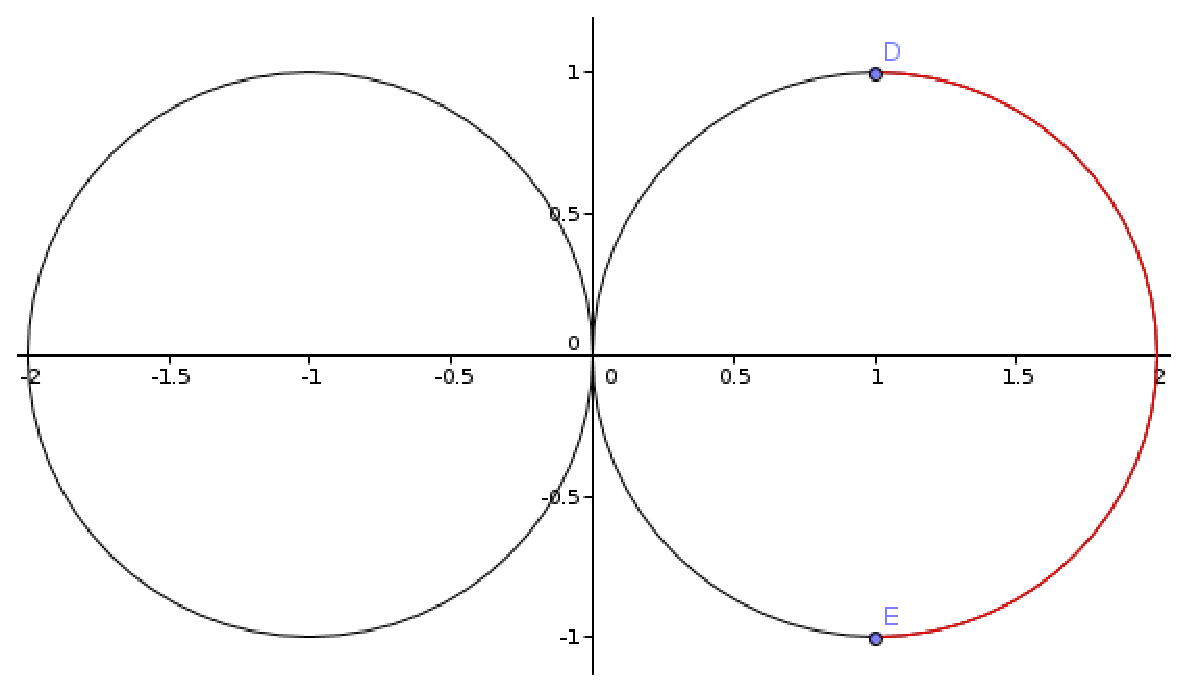
\includegraphics[scale=0.6]{Fig8Plano.eps}
\caption{Figura ocho. El conjunto $U$ será la curva negra, mientras que el conjunto $V$ será la curva roja que une los puntos $D$ y $E$.}
\end{figure}

$C(-1,1)\cong S^1$ es un retracto por deformación fuerte de $U$, mientras que $V \cong I$, que es un conjunto convexo. Por tanto, se tiene que $$H_*(U)=H_*(S^1); \quad H_*(V)=H_*(I)=H_*(\{0\})$$ Por otro lado, $U \cap V$ es la unión disjunta de dos segmentos, por lo que $$H*(U \cap V)\cong H_*(I)^2 \cong H_*(0)^2$$

Para $n > 1$, se tiene la sucesión exacta corta
\[\begin{array}{ccccccc}
H_n(U \cap V)	&\xrightarrow{g_*}	&H_n(U)\oplus H_n(V)	&\xrightarrow{h_*}	&H_n(8)		&\xrightarrow{\Delta}&H_{n-1}(U \cap V)\\
\downarrow		&					&\downarrow			&					&\downarrow	&					&\downarrow\\
0		&\rightarrow			&0			&\rightarrow			&H_n(8)		&\rightarrow			&0
\end{array}\]
donde las flechas verticales indican isomorfismos.
\\

Por exactitud, se tiene que
$$0=\im h_*\cong \frac{H_n(8)}{\ker h_*}=\frac{H_n(8)}{\im g_*}\cong H_n(8)$$

Consideremos ahora el sigueinte tramo de la sucesión de Mayer-Vietoris asociada a este recubrimiento, donde las flechas verticales indican isomorfismos.
\[\begin{array}{ccccccc}
H_1(U \cap V)	&\xrightarrow{g_1}	&H_1(U)\oplus H_1(V)	&\xrightarrow{h_1}	&H_1(8)		&\xrightarrow{\Delta_1}&H_0(U \cap v)\\
\downarrow		&					&\downarrow			&					&\downarrow	&					&\downarrow\\
0		&\rightarrow			&\mb{Z}			&\rightarrow			&H_1(8)		&\rightarrow			&\mb{Z}^2
\end{array}\]

Por exactitud, se tiene que $0=\im g_1=\ker h_1$, luego $$\mb{Z} \cong \frac{\mb{Z}^2}{\ker h_1} \cong \im h_1 =\ker \Delta_1$$

Consideremos ahora el sigueinte tramo de la sucesión de Mayer-Vietoris asociada a este recubrimiento, donde las flechas verticales indican isomorfismos.
\[\begin{array}{ccccccc}
H_0(U \cap V)	&\xrightarrow{g_0}	&H_0(U)\oplus H_0(V)	&\xrightarrow{h_0}	&H_0(8)		&\rightarrow&0\\
\downarrow		&					&\downarrow			&					&\downarrow	&					&\downarrow\\
\mb{Z}^2		&\rightarrow			&\mb{Z}^2			&\rightarrow			&\mb{Z}		&\rightarrow			&0
\end{array}\]

Por exactitud, se tiene que
\ecua{\label{Homo1Fig8}\frac{H_1(8)}{\ker \Delta_1} \cong \im \Delta_1 =\ker g_0}
$$\mb{Z} \cong \im h_0 \cong \frac{\mb{Z}^2}{\ker h_0} \implies \mb{Z} \cong \ker h_0 = \im g_0 \cong \frac{\mb{Z}^2}{\ker g_0}$$ de donde se sigue que $\ker g_0\cong \mb{Z}$.
\\

Aplicando este hecho a (\ref{Homo1Fig8}), concluimos que $$\mb{Z} \cong \frac{H_1(8)}{\mb{Z}} \quad\therefore\quad H_1(8) \cong \mb{Z}^2$$

\begin{teo}\label{HomoOcho}
\[\begin{array}{ccc}
H_n(8)\cong
\begin{cases}
\mb{Z}		&\mbox{ si }n =0\\
\mb{Z}^2	&\mbox{ si }n =1\\
0     &\mbox{ si }n \geq 2
\end{cases}
&\implies&
\beta_n(8)=
\begin{cases}
1 &\mbox{ si }n = 0\\
2 &\mbox{ si }n = 1\\
0 &\mbox{ si }n \geq 2
\end{cases}
\end{array}\]
$$\chi(8)=\beta_0(8)-\beta_1(8)=1-2=-1$$
\end{teo}

\subsection{La rosa del topólogo}
La figura ocho se puede construir de la forma siguiente: sea $p \in \mbR^2$ un punto e $I_1=[a_1,b_1], I_2=[a_2,b_2] \subset \mbR$ dos intervalos acotados. Si \[R=\partial I_1\cup \partial I_2\cup \{p\}\] se tiene que la figura ocho antes descrita se puede representar como \[\frac{I_1\sqcup\{p\}\sqcup I_2}{R}\]

Podemos extender esta construcción para añadir tantos lóbulos como queramos, de forma que conseguimos una figura llamada \textbf{rosa} o \textbf{buqué}.
\\

Sea $n > 0$ e $I_1=[a_1,b_1], \dots, I_n=[a_n,b_n] \subset \mbR$ una familia de intervalos acotados. Se define la rosa de $n$ pétalos ($B_n$) de la forma siguiente:
\[J_1=I_1\sqcup \{p\} \quad\land\quad R_1=\{p\}\cup \partial I_1 \implies B_1=\frac{J_1}{R_1}\cong S^1\]
\[J_2=J_1 \sqcup I_2 \quad\land\quad R_2=R_1 \cup \partial I_2 \implies B_2=\frac{J_2}{R_2} \cong 8\]
Esto crea una recurrencia que nos lleva a la definición de $B_n$, la rosa de $n$ pétalos: \[J_n=J_{n-1}\sqcup I_n \quad\land\quad R_n=R_{n-1}\cup \partial I_n \implies B_n=\frac{J_n}{R_n}\]

Hasta ahora, sabemos que
\[H_n(B_1)\cong
\begin{cases}
\mb{Z}		&\mbox{ si }n =0\\
\mb{Z}	&\mbox{ si }n =1\\
0     &\mbox{ si }n \geq 2
\end{cases}
\quad
H_n(B_2)\cong
\begin{cases}
\mb{Z}		&\mbox{ si }n =0\\
\mb{Z}^2	&\mbox{ si }n =1\\
0     &\mbox{ si }n \geq 2
\end{cases}
\]

Uno podría aventurarse a decir que cada pétalo de $B_p$ añade un nuevo generador al orden de homología de orden 1, y que el grupo de homología de orden $n > 1$ siempre es cero. Dado que lo tenemos confirmado para $p=1$ y $p=2$, podemos conjeturar cuál será el grupo de homología de orden 1 de $B_p$ para cualquier $p$.
\\

\textbf{Hipótesis de inducción:} Dado un $p$ natural,
\[\begin{array}{ccc}
H_n(B_p)\cong
\begin{cases}
\mb{Z}		&\mbox{ si }n =0\\
\mb{Z}^p	&\mbox{ si }n =1\\
0     &\mbox{ si }n \geq 2
\end{cases}
&\implies&
\beta_n(B_p)=
\begin{cases}
1 &\mbox{ si }n = 0\\
p &\mbox{ si }n = 1\\
0 &\mbox{ si }n \geq 2
\end{cases}
\end{array}\]

Consideremos entonces la rosa de $p+1$ pétalos, $B=B_{p+1}$. Definimos el recubrimiento de $B$ de la forma siguiente: tomamos un intervalo $I_j$ de los que conforman la rosa y dos puntos $p < q \in \mbox{int}(I_j)$. Se definen entonces los conjuntos $U=I_j$ y $V=B-[p,q]$.

\begin{figure}[h]
\centering
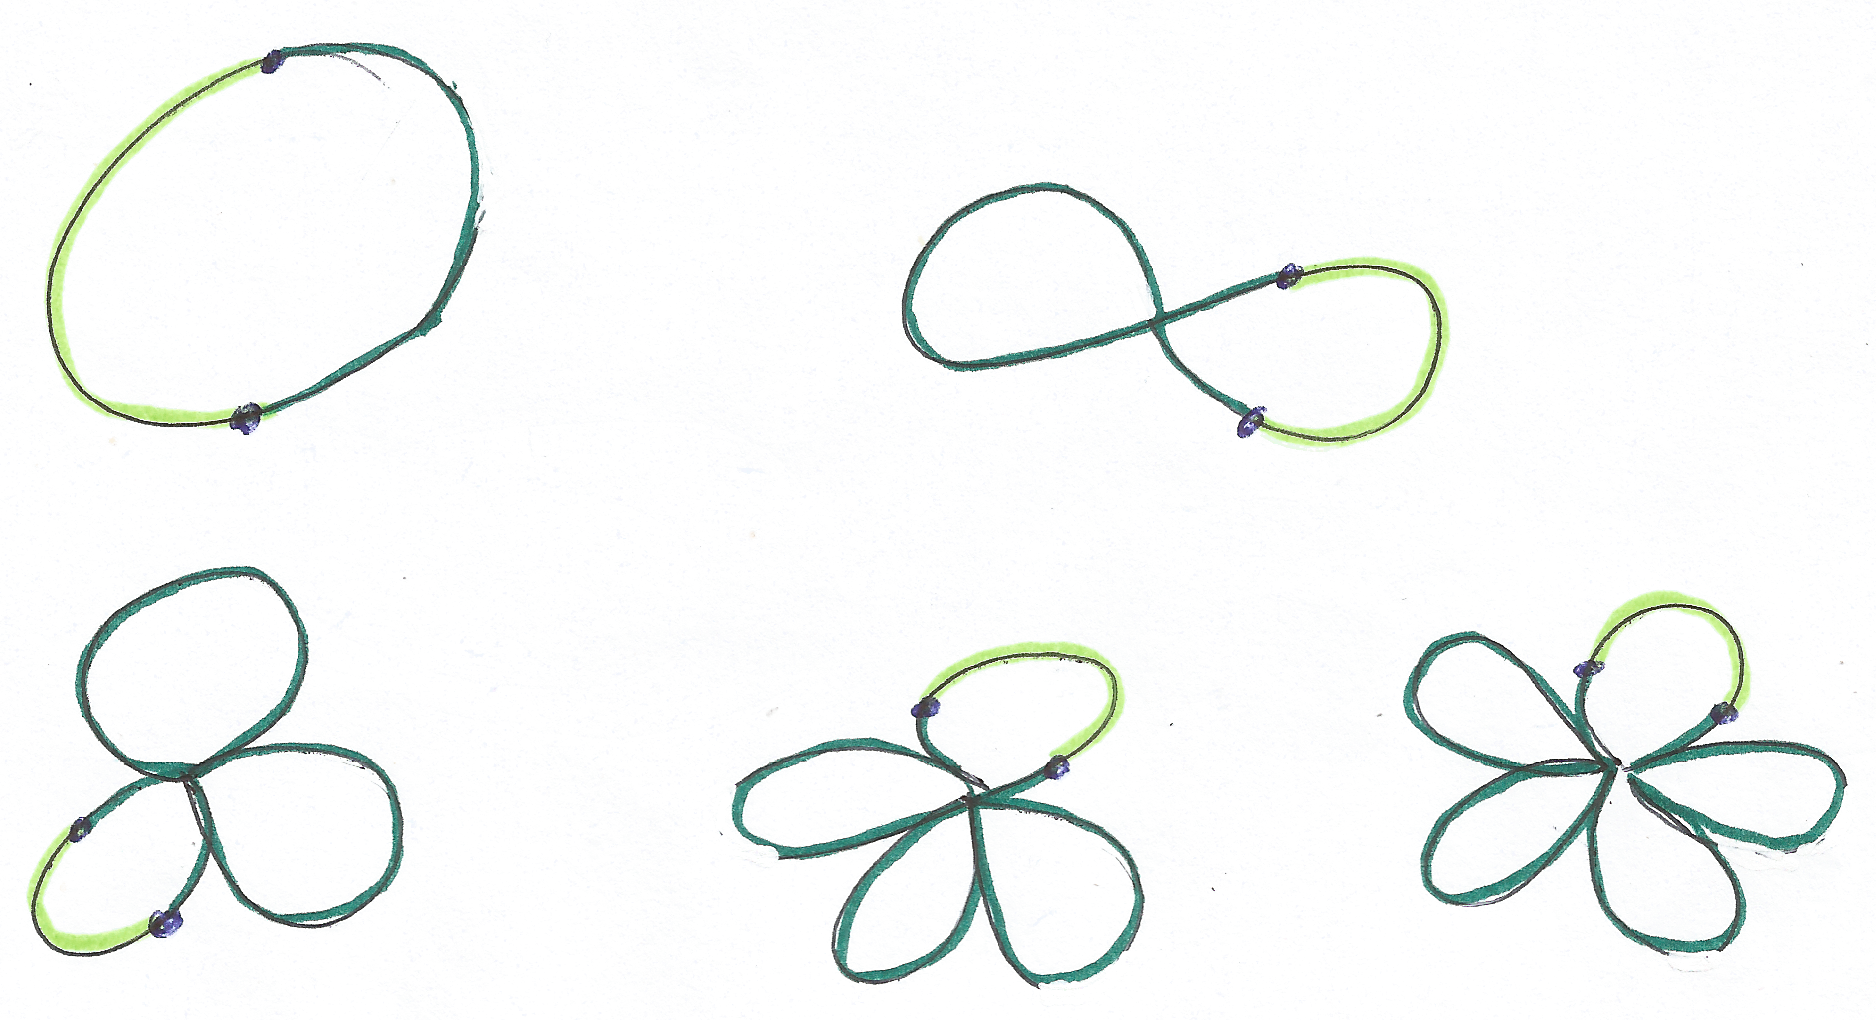
\includegraphics[scale=0.8]{Figures/Rosa}
\caption{Ejemplo de recubrimiento de la rosa de $p$ pétalos para $p=1,\dots,5$.}
\end{figure}

Observar que el espacio puntual $\{\star\}$ es un RDF de $U$, $B_p$ es un RDF de $V$ y que $\{\star\}\sqcup\{\star\}$ un RDF de $U\cap V$.
\\

Para $n > 1$, se tiene la sucesión exacta corta
\[\begin{array}{ccccccc}
H_n(U \cap V)	&\xrightarrow{g_*}	&H_n(U)\oplus H_n(V)	&\xrightarrow{h_*}	&H_n(B)		&\xrightarrow{\Delta}&H_{n-1}(U \cap V)\\
\downarrow		&					&\downarrow			&					&\downarrow	&					&\downarrow\\
0		&\rightarrow			&0			&\rightarrow			&H_n(B)		&\rightarrow			&0
\end{array}\]

Por exactitud, se tiene que $\ker \Delta=0$ y $\im \Delta=0=H_{n-1}(U\cap V)$, por lo que $\Delta$ es un isomorfismo. Se sigue que $$H_n(B) \cong H_{n-1}(U\cap V)=0$$

Consideremos ahora el sigueinte tramo de la sucesión de Mayer-Vietoris asociada a este recubrimiento:
\[\begin{array}{ccccccc}
H_0(U \cap V)	&\xrightarrow{g_0}	&H_0(U)\oplus H_0(V)	&\xrightarrow{h_0}	&H_0(B)		&\rightarrow&0\\
\downarrow		&					&\downarrow			&					&\downarrow	&					&\downarrow\\
\mb{Z}^2		&\rightarrow			&\mb{Z}^2			&\rightarrow			&\mb{Z}		&\rightarrow			&0
\end{array}\]

Por exactitud, se tiene que $\im h_0 \cong \mb{Z}$, por lo que $\im g_0=\ker h_0 \cong \mb{Z}$. De aquí se sigue que $\im \Delta_1=\ker g_0 \cong \mb{Z}$.
\\

Consideremos ahora el sigueinte tramo de la sucesión de Mayer-Vietoris asociada a este recubrimiento.
\[\begin{array}{ccccccc}
H_1(U \cap V)	&\xrightarrow{g_1}	&H_1(U)\oplus H_1(V)	&\xrightarrow{h_1}	&H_1(B)		&\xrightarrow{\Delta_1}&H_0(U \cap v)\\
\downarrow		&					&\downarrow			&					&\downarrow	&					&\downarrow\\
0		&\rightarrow			&\mb{Z}^p			&\rightarrow			&	H_1(B)	&\rightarrow			&\mb{Z}^2
\end{array}\]

Por exactitud, se tiene que $\ker h_1=\im g_1=0$, por lo que $\ker \Delta_1=\im h_1\cong \mb{Z}^p$. Como ya sabemos que $\im \Delta_1 \cong \mb{Z}$, se sigue que $$\frac{H_1(B)}{\mb{Z}^p} \cong \frac{H_1(B)}{\ker \Delta_1} \cong \im \Delta_1 \cong \mb{Z} \implies H_1(B)\cong \mb{Z}^{p+1}$$

Esto confirma nuestra conjetura. Además, $$\chi(B_p)=\beta_0(B_p)-\beta_1(B_p)=1-p$$

\section{Grupo de homología del toro}
El \textbf{toro paramétrico} se define como la superficie de ecuación implícita $$z^2+\left(R-\sqrt{x^2+y^2}\right)^2=r^2; \quad 0 < r < R$$ Podemos considerar un recubrimiento del toro paramétrico formado por dos cilindros que se solapan, $U$ y $V$, como los mostrados en la figura \ref{ToroUV}.
\\

\begin{figure}[h]
\centering
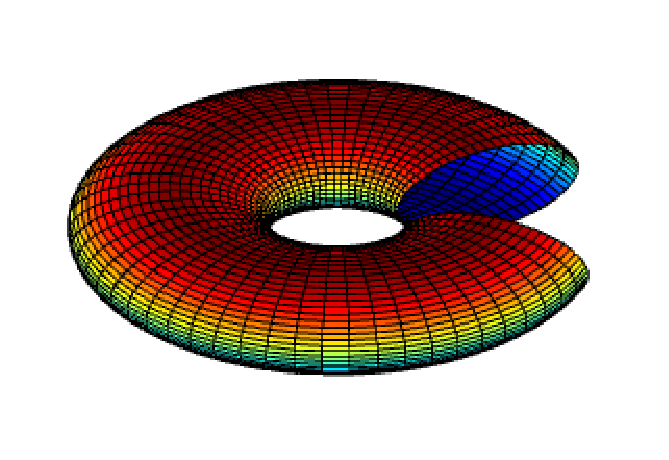
\includegraphics[scale=0.6]{ToroU.eps}
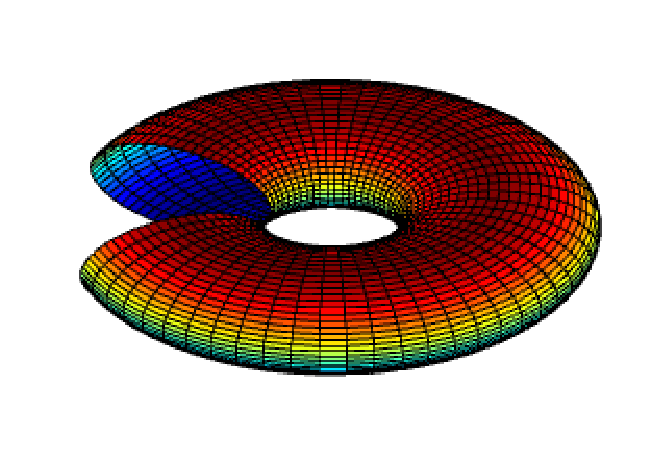
\includegraphics[scale=0.6]{ToroV.eps}
\caption{\label{ToroUV} Las figuras $U$ y $V$. Notar que $S^1$ es un retracto por deformación fuerte de ambas figuras.}
\end{figure}

Dado que $S^1$ es un retracto por deformación fuerte de $U$ y de $V$, se tiene que $$H_*(U) \cong H_*(S^1)\cong H_*(V)$$

Por otro lado, $U\cap V$ posee dos arcocomponentes, $C_1$ y $C_2$, por lo que la proposición \ref{SumaDirArco} nos dice que$ H_*(U\cap V) \cong H_*(C_1)\oplus H_*(C_2)$. Como $S^1$ es un retracto por deformación fuerte de $C_1$ y de $C_2$, se sigue que $$H_*(C_1)\oplus H_*(C_2) \cong H_*(S^1)\oplus H_*(S^1)\cong H_*(S^1)^2$$

Sea $n > 2$. Considérese la siguiente sucesión exacta, donde las flechas verticales indican isomorfismos.

\[\begin{array}{ccccccc}
H_n(U \cap V)	&\xrightarrow{g_*}	&H_n(U)\oplus H_n(V)	&\xrightarrow{h_*}	& H_n(T)		&\xrightarrow{\Delta}&H_{n-1}(U \cap v)\\
\downarrow		&					&\downarrow			&					&\downarrow	&					&\downarrow\\
0				&\rightarrow			&0					&\rightarrow			&H_n(T)		&\rightarrow			&0
\end{array}\]

Dado que esta sucesión es exacta, podemos afirmar que $\ker \Delta=\im h_*=0$ y $\im \Delta \leq 0$, por lo que $$H_n(T) \cong \frac{H_n(T)}{\ker \Delta} \cong \im \Delta \leq 0 \implies H_n(T)=0$$

\noindent\textbf{Cálculo de $H_2(T)$}
\\
Considérese la siguiente sucesión exacta, donde las flechas verticales indican isomorfismos.
\[\begin{array}{ccccccc}
H_0(U \cap V)	&\xrightarrow{g_0}	&H_0(U)\oplus H_0(V)	&\xrightarrow{h_0}	&H_0(T)		&\xrightarrow{f}&0\\
\downarrow		&					&\downarrow			&					&\downarrow	&					&\downarrow\\
\mb{Z}^2			&\rightarrow			&\mb{Z}^2			&\rightarrow			&\mb{Z}		&\rightarrow			&0
\end{array}\]

Dado que esta sucesión es exacta, podemos afirmar que $\im h_0=\ker f \cong \mb{Z}$ y $\im g_0=\ker h_0\cong \mb{Z}$, luego $$\frac{\mb{Z}^2}{\ker h_0} \cong \im h_0 \cong \mb{Z} \implies \ker h_0\cong\mb{Z}$$ $$\frac{\mb{Z}^2}{\ker g_0} \cong \im g_0 \cong \mb{Z} \implies \ker g_0\cong\mb{Z}$$

Considérese el siguiente tramo de la sucesión de Mayer-Vietoris asociada a este recubrimiento, donde las flechas verticales indican isomorfismos.
\[\begin{array}{ccccccc}
H_1(U \cap V)	&\xrightarrow{g_1}	&H_1(U)\oplus H_1(V)	&\xrightarrow{h_1}	&H_1(T)		&\xrightarrow{\Delta_1}&H_0(U \cap V)\\
\downarrow		&					&\downarrow			&					&\downarrow	&					&\downarrow\\
\mb{Z}^2			&\rightarrow			&\mb{Z}^2			&\rightarrow			&H_1(T)		&\rightarrow			&\mb{Z}^2
\end{array}\]

Dado que la sucesión es exacta,
$$\frac{H_1(T)}{\ker \Delta_1}\cong \im \Delta_1=\ker g_0\cong \mb{Z}$$

Considérese el siguiente tramo de la sucesión de Mayer-Vietoris asociada a este recubrimiento, donde las flechas verticales indican isomorfismos.
\[\begin{array}{ccccccc}
H_2(U \cap V)	&\xrightarrow{g_2}	&H_2(U)\oplus H_2(V)	&\xrightarrow{h_2}	& H_2(T)		&\xrightarrow{\Delta_2}&H_1(U \cap v)\\
\downarrow		&					&\downarrow			&					&\downarrow	&					&\downarrow\\
0				&\rightarrow			&0					&\rightarrow			&H_2(T)		&\rightarrow			&\mb{Z}^2
\end{array}\]

Dado que la sucesión es exacta,
$$H_2(T) \cong \frac{H_2(T)}{\im h_2}=\frac{H_2(T)}{\ker \Delta_2} \cong \im \Delta_2=\ker g_1$$

Recordemos cómo se define $g_*$: $$\funcio{g_*}{H_1(C_1\sqcup C_2)}{H_1(U)\oplus H_1(V)}{[c]}{([c],[-c])}$$ Sea $[c] \in \ker g_*$. Dado que $S^1$ es un retracto por deformación fuerte del cilindro, existen ciclos $x,y \in Z_1(S^1)$ tales que $$H_1(C_1\sqcup C_2)\cong H_1(S^1)\oplus H_1(S^1)=([x])_\mb{Z}\oplus ([y])_\mb{Z}$$ de forma que $c=\alpha x+\beta y$ para algunos $\alpha,\beta$ enteros.
\\

Considérense ahora las inclusiones $i: U \cap V \hookrightarrow U$ y $j: U \cap V \hookrightarrow V$. Se tiene que $$0=g_*([c])=([c],-[c])=(i_*[c],-j_*[c]) \iff \begin{cases}i_*([c])=0\\j_*([c])=0\end{cases}$$ Dado que $x$ e $y$ son símplices homólogos en $U$, $$i_*([c])=i_*([\alpha x+\beta y])=i_*([\alpha x+\beta x])=(\alpha+\beta)i_*([x])=0 \iff \alpha=-\beta$$ Se sigue que $$H_2(T)\cong \ker g_*=\{[\alpha x-\alpha y]: \alpha \in \mb{Z}\}=([x-y])_\mb{Z}\cong \mb{Z}$$

\noindent\textbf{Cálculo de $H_1(T)$}
\\
Considérese la siguiente relación de equivalencia sobre $I^2$: $$\forall s,t \in [0,1] \quad (s,0) \sim (s,1) \land (0,t) \sim (1,t)$$ El espacio cociente $T_C=I^2/\sim$ se denomina \textbf{toro llano}, y es homeomorfo al toro paramétrico. Si $p=(1/2,1/2)$, $I^2-\{p\}$ es deformable en $\partial(I^2)$, por lo que $\partial(I^2)$ es un retracto por deformación de $I^2-\{p\}$.
\\

Se puede definir una retracción que sea compatible con la relación de equivalencia $\sim$, de forma que $\partial T_C$ es un retracto por deformación del toro llano. Esta figura es homeomorfa a la figura ocho, como puede verse en la figura \ref{fig8}.
\\

\begin{figure}[h]
\centering
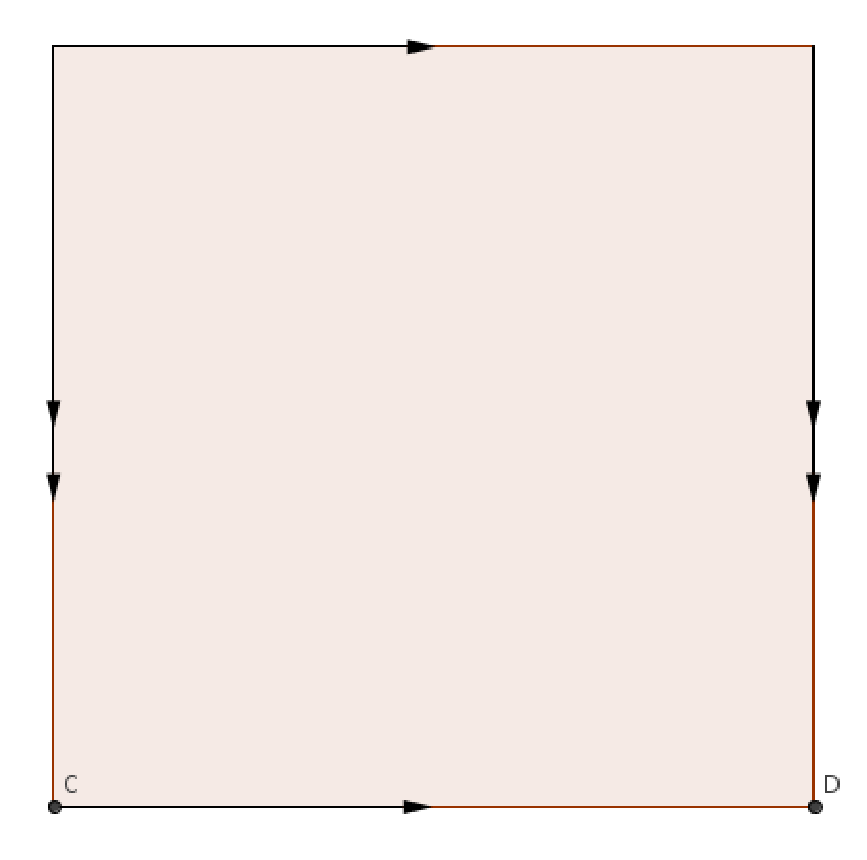
\includegraphics[scale=0.4]{Clifford.eps}\hspace{2cm}
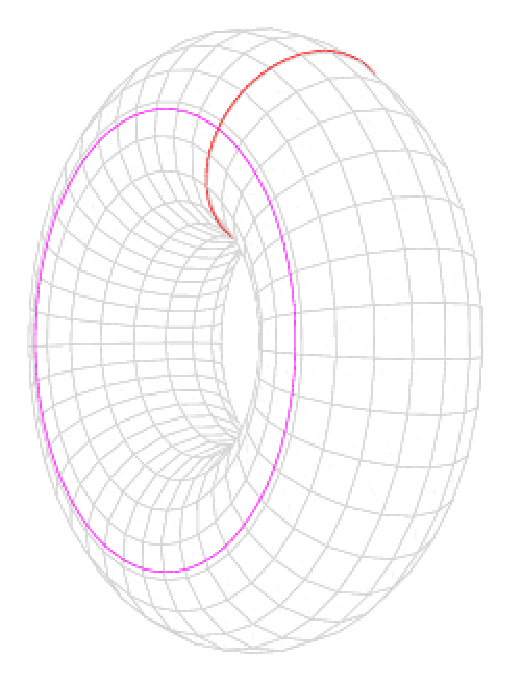
\includegraphics[scale=0.55]{FiguraOcho.eps}
\caption{\label{fig8}Izquierda: toro llano. Derecha: figura ocho proyectada sobre el toro paramétrico.}
\end{figure}

Sea ahora $V=B(p;1/4)$. Se tiene que $V \subset I^2$ y $V\cap\partial (I^2)=\emptyset$, de forma que $V$ y $U=T_C-\{p\}$ forman un recubrimiento del toro llano. Ahora bien, $U \cap V$ es una corona circular, por lo que $S^1$ es un retracto por deformación fuerte de $U \cap V$. Así, se tiene que $$H_*(T-\{p\}) \cong H_*(8); \quad H_*(V) \cong H_*(\{p\}); \quad H_*(U \cap v) \cong H_*(S^1)$$

Considérese el siguiente tramo de la sucesión de Mayer-Vietoris asociada a este recubrimiento, donde las flechas verticales indican isomorfismos.
\[\begin{array}{ccccccc}
H_2(U \cap V)	&\xrightarrow{g_2}	&H_2(U)\oplus H_2(V)	&\xrightarrow{h_2}	& H_2(T)		&\xrightarrow{\Delta_2}&H_1(U \cap V)\\
\downarrow		&					&\downarrow			&					&\downarrow	&					&\downarrow\\
0				&\rightarrow			&0					&\rightarrow			&\mb{Z}		&\rightarrow			&\mb{Z}
\end{array}\]

Dado que la sucesión es exacta, se tiene que $0=\im h_2=\ker \Delta_2$, luego $$\im \Delta_2\cong \frac{H_2(T)}{\ker \Delta_2} \cong \mb{Z}$$

Considérese el siguiente tramo de la sucesión de Mayer-Vietoris asociada a este recubrimiento, donde las flechas verticales indican isomorfismos.
\[\begin{array}{ccccccc}
H_1(U \cap V)	&\xrightarrow{g_1}	&H_1(U)\oplus H_1(V)	&\xrightarrow{h_1}	&H_1(T)		&\xrightarrow{\Delta_1}&H_0(U \cap V)\\
\downarrow		&					&\downarrow			&					&\downarrow	&					&\downarrow\\
\mb{Z}		&\rightarrow			&\mb{Z}^2			&\rightarrow			&H_1(T)		&\rightarrow			&\mb{Z}
\end{array}\]

Dado que la sucesión es exacta, se tiene que
$\mb{Z} \cong \im \Delta_2 =\ker g_1$, luego $$0=\frac{\mb{Z}}{\ker g_1}\cong \im g_1=\ker h_1 \implies \mb{Z}\cong \frac{\mb{Z}}{\ker h_1}\cong \im h_1=\ker \Delta_1$$ De aquí se sigue que $\im \Delta_1 \cong H_1(T)/\ker \Delta_1\cong H_1(T)/\mb{Z}$.
\\

Considérese el siguiente tramo de la sucesión de Mayer-Vietoris asociada a este recubrimiento, donde las flechas verticales indican isomorfismos.
\[\begin{array}{ccccccc}
H_0(U \cap V)	&\xrightarrow{g_0}	&H_0(U)\oplus H_0(V)	&\xrightarrow{h_0}	&H_0(T)		&\rightarrow&0\\
\downarrow		&					&\downarrow			&					&\downarrow	&					&\downarrow\\
\mb{Z}^2		&\rightarrow			&\mb{Z}^2			&\rightarrow			&\mb{Z}		&\rightarrow			&0
\end{array}\]

Ya tenemos toda la información necesaria para poder determinar $H_1(T)$: $$\mb{Z} \cong \im h_0 \cong \frac{\mb{Z}^2}{\ker h_0} \implies \ker h_0 \cong \mb{Z}$$
$$\mb{Z} \cong \ker h_0 =\im g_0 \cong \frac{\mb{Z}^2}{\ker g_0} \implies \ker g_0\cong \mb{Z}$$
$$\mb{Z} \cong \ker g_0 =\im \Delta_1 \cong \frac{H_1(T)}{\mb{Z}} \therefore H_1(T)\cong \mb{Z}^2$$

\begin{teo}\label{HomoToro}
\[\begin{array}{ccc}
H_n(T)=
\begin{cases}
\mb{Z}		&\mbox{ si }n =0,2\\
\mb{Z}^2	&\mbox{ si }n =1\\
0     &\mbox{ si }n > 2
\end{cases}
&\implies&
\beta_n(T)=
\begin{cases}
1 &\mbox{ si }n = 0,2\\
2 &\mbox{ si }n = 1\\
0 &\mbox{ si }n > 2
\end{cases}
\end{array}\]
Y esto nos lleva a un hecho que ya sabíamos: $$\chi(8)=\beta_0(T)-\beta_1(T)+\beta_2(T)=1-2+1=0$$
\end{teo}
